\section{Using Tor?}

Tor is a system intended to enable online anonymity, composed of client
software and a network of servers which can hide information about
users' locations and other factors which might identify them. Imagine a
message being wrapped in several layers of protection: every server
needs to take off one layer, thereby immediately deleting the sender
information of the previous server.

Use of this system makes it more difficult to trace internet traffic to
the user, including visits to Web sites, online posts, instant messages,
and other communication forms. It is intended to protect users' personal
freedom, privacy, and ability to conduct confidential business, by
keeping their internet activities from being monitored. The software is
open-source and the network is free of charge to use.

Like all current low latency anonymity networks, Tor cannot and does not
attempt to protect against monitoring of traffic at the boundaries of
the Tor network, i.e., the traffic entering and exiting the network.
While Tor does provide protection against traffic analysis, it cannot
prevent traffic confirmation (also called end-to-end correlation)

Caution: As Tor does not, and by design cannot, encrypt the traffic
between an exit node and the target server, any exit node is in a
position to capture any traffic passing through it which does not use
end-to-end encryption such as TLS. (If your postman is corrupt he might
still open the envelope and read the content). While this may or may not
inherently violate the anonymity of the source, if users mistake Tor's
anonymity for end-to-end encryption they may be subject to additional
risk of data interception by third parties. So: the location of the user
remains hidden; however, in some cases content is vulnerable for
analysis through which also information about the user may be gained.

\subsection{Using Tor Browser Bundle}

The Tor Browser Bundle lets you use Tor on Windows, OSX and/or Linux
without requiring you to configure a Web browser. Even better, it's also
a portable application that can be run from a USB flash drive, allowing
you to carry it to any PC without installing it on each computer's hard
drive.

\subsection{Downloading Tor Browser Bundle}

You can download the Tor Browser Bundle from the torproject.org Web site
(\href{https://www.torproject.org}{https://www.torproject.org}), either
as a single file (13MB) or a split version that is multiple files of 1.4
MB each which may proof easier to download on slow connections.

If the torproject.org Web site is filtered from where you are, type
``tor mirrors'' in your favorite Web search engine: The results probably
include some alternative addresses to download the Tor Browser Bundle.

Caution: When you download Tor Bundle (plain or split versions), you
should check the signatures of the files, especially if you are
downloading the files from a mirror site. This step ensures that the
files have not been tampered with. To learn more about signature files
and how to check them, read
\href{https://www.torproject.org/docs/verifying-signatures}{https://www.torproject.org/docs/verifying-signatures}

(You can also download the GnuPG software that you will need to check
the signature here:
\href{http://www.gnupg.org/download/index.en.html\#auto-ref-2}{http://www.gnupg.org/download/index.en.html\#auto-ref--2})

The instructions below refer to installing Tor Browser on Microsoft
Windows. If you are using a different operating system, refer to the
torproject.org website for download links and instructions.

\subsubsection{Installing from a single file}

\begin{enumerate}[1.]
\item
  In your Web browser, enter the download URL for Tor Browser:
  \href{https://www.torproject.org/download/download}{https://www.torproject.org/download/download}
\end{enumerate}
\begin{figure}[htbp]
\centering
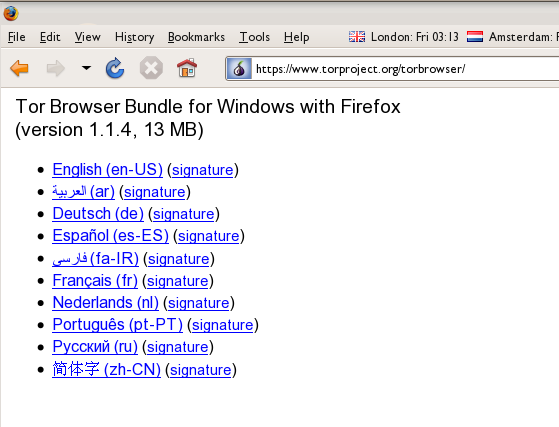
\includegraphics{tor_1.png}
\caption{Tor}
\end{figure}

\begin{enumerate}[1.]
\setcounter{enumi}{1}
\item
  Click the link for your language to download the installation file.
\item
  On windows double-click the .EXE file you just downloaded. A ``7-Zip
  self-extracting archive'' window appears.
\end{enumerate}
\begin{figure}[htbp]
\centering
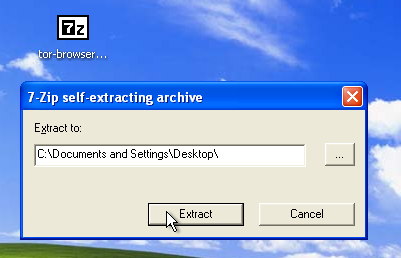
\includegraphics{tor_2.png}
\caption{Tor}
\end{figure}

\begin{enumerate}[1.]
\setcounter{enumi}{3}
\item
  Choose a folder into which you want to extract the files and click
  ``Extract''.
\end{enumerate}
\textbf{Note:} You can choose to extract the files directly onto a USB
key or memory stick if you want to use Tor Browser on different
computers (for instance on public computers in Internet cafes).

\begin{enumerate}[1.]
\setcounter{enumi}{4}
\item
  When the extraction is completed, open the folder and check that the
  contents match the image below:
\end{enumerate}
\begin{figure}[htbp]
\centering
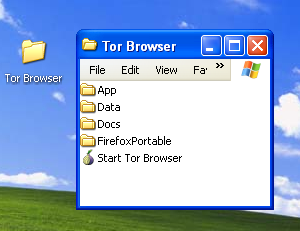
\includegraphics{tor_3.png}
\caption{Tor}
\end{figure}

\begin{enumerate}[1.]
\setcounter{enumi}{5}
\item
  To clean up, delete the .EXE file you originally downloaded.
\end{enumerate}
\subsubsection{Installing from split files}

\begin{enumerate}[1.]
\item
  In your Web browser, enter the URL for the split version of the Tor
  Browser Bundle (https://www.torproject.org/torbrowser/split.html),
  then click the link for your language to get to a page that looks like
  the one for English below:
\end{enumerate}
\begin{figure}[htbp]
\centering
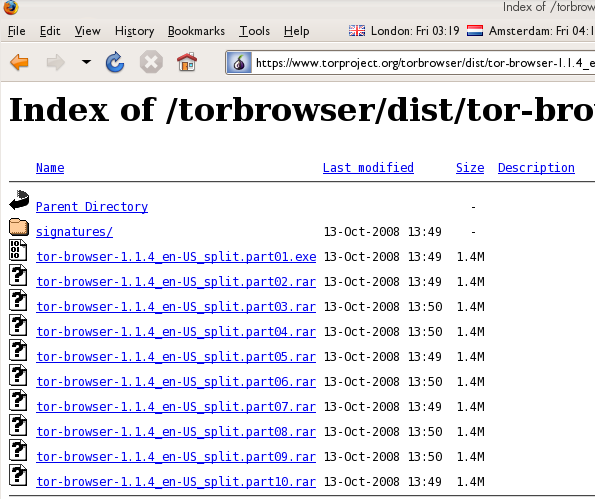
\includegraphics{tor_4.png}
\caption{Tor}
\end{figure}

\begin{enumerate}[1.]
\setcounter{enumi}{1}
\item
  Click each file to download it (one ending in ``.exe'' and nine others
  ending in ``.rar''), one after the other, and save them all in one
  folder on your hard- or USB-drive.
\item
  Double-click the first part (the file whose name ends in ``.exe'').
  This runs a program to gather all the parts together.
\end{enumerate}
\begin{figure}[htbp]
\centering
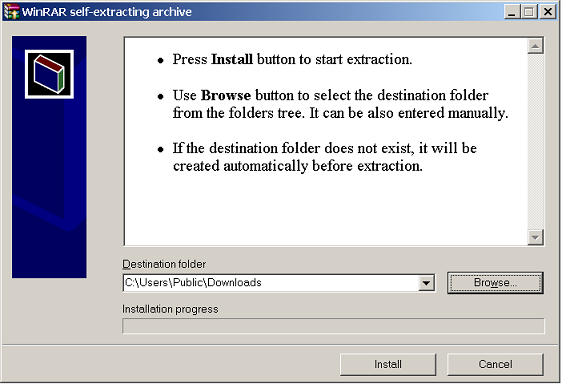
\includegraphics{tor_5.png}
\caption{Tor}
\end{figure}

\begin{enumerate}[1.]
\setcounter{enumi}{3}
\item
  Choose a folder where you want to install the files, and click
  ``Install''. The program displays messages about its progress while
  it's running, and then quits.
\item
  When the extraction is completed, open the folder and check that the
  contents match the image below:
\end{enumerate}
\begin{figure}[htbp]
\centering
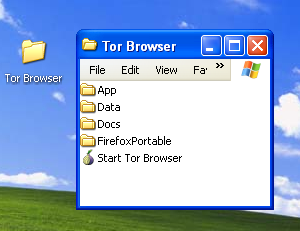
\includegraphics{tor_6.png}
\caption{Tor}
\end{figure}

\begin{enumerate}[1.]
\setcounter{enumi}{5}
\item
  To clean up, delete all the files you originally downloaded.
\end{enumerate}
\subsection{Using Tor Browser}

Before you start:

\begin{itemize}
\item
  \textbf{Close Firefox.} If Firefox is installed on your computer, make
  sure it is not currently running.
\item
  \textbf{Close Tor.} If Tor is already installed on your computer, make
  sure it is not currently running.
\end{itemize}
Launch Tor Browser:

\begin{enumerate}[1.]
\item
  In the ``Tor Browser'' folder, double-click ``Start Tor Browser''. The
  Tor control panel (``Vidalia'') opens and Tor starts to connect to the
  Tor network.
\end{enumerate}
\begin{figure}[htbp]
\centering
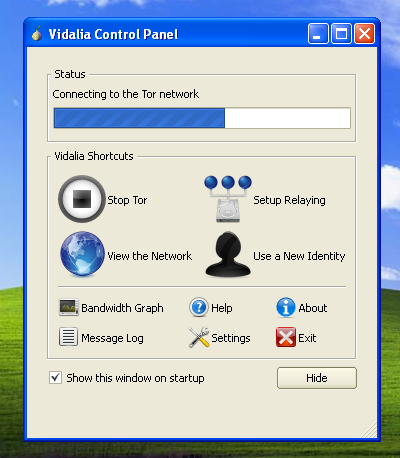
\includegraphics{tor_7.png}
\caption{Tor}
\end{figure}

\begin{enumerate}[1.]
\setcounter{enumi}{1}
\item
  When a connection is established, Firefox automatically connects to
  the TorCheck page and then confirms if you are connected to the Tor
  network. This may take some time, depending on the quality of your
  Internet connection.
\end{enumerate}
\begin{figure}[htbp]
\centering
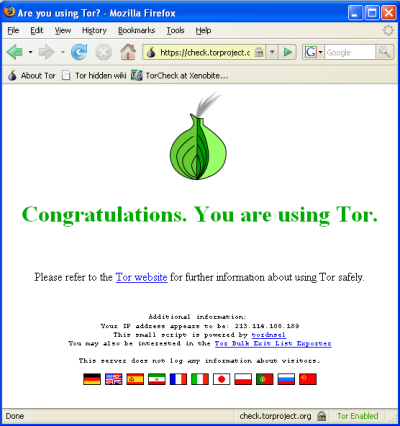
\includegraphics{tor_8.png}
\caption{Tor}
\end{figure}

\begin{enumerate}[1.]
\setcounter{enumi}{2}
\item
  If you are connected to the Tor network, a green onion icon appears in
  the System Tray on the lower-right-hand corner of your screen:
\end{enumerate}
\begin{figure}[htbp]
\centering

\includegraphics{tor_9.png}
\caption{Tor}
\end{figure}

\subsection{Browsing the Web using Tor Browser}

Try viewing a few Web sites, and see whether they display. The sites are
likely to load more slowly than usual because your connection is being
routed through several relays.

\subsection{If this does not work}

If the onion in the Vidalia Control Panel never turns green or if
Firefox opened, but displayed a page saying ``Sorry. You are not using
Tor'', as in the image below, then you are not using Tor.

\begin{figure}[htbp]
\centering

\includegraphics{tor_10.png}
\caption{Tor}
\end{figure}

If you see this message, close Firefox and Tor Browser and then repeat
the steps above. You can perform this check to ensure that you are using
tor, at any time by clicking the bookmark button labelled ``TorCheck at
Xenobite\ldots{}'' in the Firefox toolbar.

If Firefox browser does not launch, another instance of the browser may
be interfering with Tor Browser. To fix this:

\begin{enumerate}[1.]
\item
  Open the Windows Task Manager. How you do this depends on how your
  computer is set up. On most systems, you can right-click in the Task
  Bar and then click ``Task Manager''.
\item
  Click the ``Processes'' tab.
\item
  Look for a process in the list named ``firefox.exe''.
\item
  If you find one, select the entry and click ``End Process''.
\item
  Repeat the steps above to launch Tor Browser.
\end{enumerate}
If Tor Browser still doesn't work after two or three tries, Tor may be
partly blocked by your ISP and you should try using the \textbf{bridge}
feature of Tor.
